\documentclass[journal,12pt,twocolumn]{IEEEtran}

\usepackage{setspace}
\usepackage{gensymb}
\singlespacing
\usepackage[cmex10]{amsmath}

\usepackage{amsthm}

\usepackage{mathrsfs}
\usepackage{txfonts}
\usepackage{stfloats}
\usepackage{bm}
\usepackage{cite}
\usepackage{cases}
\usepackage{subfig}

\usepackage{longtable}
\usepackage{multirow}

\usepackage{enumitem}
\usepackage{mathtools}
\usepackage{steinmetz}
\usepackage{tikz}
\usepackage{circuitikz}
\usepackage{verbatim}
\usepackage{tfrupee}
\usepackage[breaklinks=true]{hyperref}
\usepackage{graphicx}
\usepackage{tkz-euclide}

\usetikzlibrary{calc,math}
\usepackage{listings}
    \usepackage{color}                                            %%
    \usepackage{array}                                            %%
    \usepackage{longtable}                                        %%
    \usepackage{calc}                                             %%
    \usepackage{multirow}                                         %%
    \usepackage{hhline}                                           %%
    \usepackage{ifthen}                                           %%
    \usepackage{lscape}     
\usepackage{multicol}
\usepackage{chngcntr}

\DeclareMathOperator*{\Res}{Res}

\renewcommand\thesection{\arabic{section}}
\renewcommand\thesubsection{\thesection.\arabic{subsection}}
\renewcommand\thesubsubsection{\thesubsection.\arabic{subsubsection}}

\renewcommand\thesectiondis{\arabic{section}}
\renewcommand\thesubsectiondis{\thesectiondis.\arabic{subsection}}
\renewcommand\thesubsubsectiondis{\thesubsectiondis.\arabic{subsubsection}}


\hyphenation{op-tical net-works semi-conduc-tor}
\def\inputGnumericTable{}                                 %%

\lstset{
%language=C,
frame=single, 
breaklines=true,
columns=fullflexible
}
\begin{document}


\newtheorem{theorem}{Theorem}[section]
\newtheorem{problem}{Problem}
\newtheorem{proposition}{Proposition}[section]
\newtheorem{lemma}{Lemma}[section]
\newtheorem{corollary}[theorem]{Corollary}
\newtheorem{example}{Example}[section]
\newtheorem{definition}[problem]{Definition}

\newcommand{\BEQA}{\begin{eqnarray}}
\newcommand{\EEQA}{\end{eqnarray}}
\newcommand{\define}{\stackrel{\triangle}{=}}
\bibliographystyle{IEEEtran}
\raggedbottom
\setlength{\parindent}{0pt}
\providecommand{\mbf}{\mathbf}
\providecommand{\pr}[1]{\ensuremath{\Pr\left(#1\right)}}
\providecommand{\qfunc}[1]{\ensuremath{Q\left(#1\right)}}
\providecommand{\sbrak}[1]{\ensuremath{{}\left[#1\right]}}
\providecommand{\lsbrak}[1]{\ensuremath{{}\left[#1\right.}}
\providecommand{\rsbrak}[1]{\ensuremath{{}\left.#1\right]}}
\providecommand{\brak}[1]{\ensuremath{\left(#1\right)}}
\providecommand{\lbrak}[1]{\ensuremath{\left(#1\right.}}
\providecommand{\rbrak}[1]{\ensuremath{\left.#1\right)}}
\providecommand{\cbrak}[1]{\ensuremath{\left\{#1\right\}}}
\providecommand{\lcbrak}[1]{\ensuremath{\left\{#1\right.}}
\providecommand{\rcbrak}[1]{\ensuremath{\left.#1\right\}}}
\theoremstyle{remark}
\newtheorem{rem}{Remark}
\newcommand{\sgn}{\mathop{\mathrm{sgn}}}
\providecommand{\abs}[1]{\left\vert#1\right\vert}
\providecommand{\res}[1]{\Res\displaylimits_{#1}} 
\providecommand{\norm}[1]{\left\lVert#1\right\rVert}
%\providecommand{\norm}[1]{\lVert#1\rVert}
\providecommand{\mtx}[1]{\mathbf{#1}}
\providecommand{\mean}[1]{E\left[ #1 \right]}
\providecommand{\fourier}{\overset{\mathcal{F}}{ \rightleftharpoons}}
%\providecommand{\hilbert}{\overset{\mathcal{H}}{ \rightleftharpoons}}
\providecommand{\system}{\overset{\mathcal{H}}{ \longleftrightarrow}}
\providecommand{\ztrans}{\overset{\mathcal{Z}}{ \rightleftharpoons}}
	%\newcommand{\solution}[2]{\textbf{Solution:}{#1}}
\newcommand{\solution}{\noindent \textbf{Solution: }}
\newcommand{\cosec}{\,\text{cosec}\,}
\providecommand{\dec}[2]{\ensuremath{\overset{#1}{\underset{#2}{\gtrless}}}}
\newcommand{\myvec}[1]{\ensuremath{\begin{pmatrix}#1\end{pmatrix}}}
\newcommand{\mydet}[1]{\ensuremath{}}
\numberwithin{equation}{subsection}

\makeatletter
\@addtoreset{figure}{problem}
\makeatother
\let\StandardTheFigure\thefigure
\let\vec\mathbf

\renewcommand{\thefigure}{\theproblem}

\def\putbox#1#2#3{\makebox[0in][l]{\makebox[#1][l]{}\raisebox{\baselineskip}[0in][0in]{\raisebox{#2}[0in][0in]{#3}}}}
     \def\rightbox#1{\makebox[0in][r]{#1}}
     \def\centbox#1{\makebox[0in]{#1}}
     \def\topbox#1{\raisebox{-\baselineskip}[0in][0in]{#1}}
     \def\midbox#1{\raisebox{-0.5\baselineskip}[0in][0in]{#1}}
\vspace{3cm}
\title{Gate Assignment 2}
\author{Tanmay Goyal - AI20BTECH11021}
\maketitle
\newpage
\bigskip
\renewcommand{\thefigure}{\theenumi}
\renewcommand{\thetable}{\theenumi}
Download all python codes from 
\begin{lstlisting}
https://github.com/tanmaygoyal258/EE3900-Linear-Systems-and-Signal-processing/blob/main/GateAssignment2/code.py
\end{lstlisting}
Download all latex codes from 
\begin{lstlisting}
https://github.com/tanmaygoyal258/EE3900-Linear-Systems-and-Signal-processing/blob/main/GateAssignment2/main.tex
\end{lstlisting}
\section{Problem}
(EC-2010/Q.42)The transfer function for a discrete time LTI system is given by:
\begin{align}
    H(z) = \frac{2 - \frac{3}{4}z^{-1}}{1 - \frac{3}{4}z^{-1} + \frac{1}{8}z^{-2}}
\end{align}
Consider the following statements:\\
S1: The system is stable and causal for ROC: $\abs{z} > \frac{1}{2}$\\
S2: The system is stable but not causal for ROC:  $\abs{z} < \frac{1}{4}$\\
S3: The system is neither stable nor causal for ROC:  $\frac{1}{4}<\abs{z} < \frac{1}{2}$\\
Which one of the following statement are valid?
\begin{enumerate}
    \item Both S1 and S2 are true
    \item Both S2 and S3 are true
    \item Both S1 and S3 are true
    \item S1, S2 and S3 are all true
\end{enumerate}
\section{Solution}
\begin{definition}
We say that a system is \textbf{stable} if it produces a bounded output for every possible bounded input, i.e it satisfies the BIBO(Bounded-input-Bounded-output) condition.
\end{definition}

\begin{definition}
We say that a system is \textbf{Causal} if the output of a system at a given time instance is independent of the future input values, i.e the output at a particular instance only depends on the present and past input values.
\end{definition}

\begin{lemma}
A system is said to be BIBO stable if and only if the ROC consists of the unit circle in the $Z$ plane.
\end{lemma}
\begin{lemma}
A system is causal if and only if the transfer function $h[n]$ satisfies $h[n] = 0 , n<0$
\end{lemma}
\begin{proof}
Let the input signal be given by $x[n]$ and the output signal be given by $y[n]$, then, we know in an LTI system:
\begin{align}
    y[n] = h[n] * x[n] = \sum_{k = -\infty}^\infty h[k]x[n-k]
\end{align}
Since, $y[n]$ is causal, it should be independent of future values of $n$. \\
If $k < 0$, then $n - k > n$, which is undesirable, and thus, to keep $y[n]$ independent of future values, $h[k] = 0 , k< 0$
\end{proof}
\begin{lemma}
If $x[n] = a^nu[n]$, where 
\begin{align}
    u[n] = 
    \begin{cases}
    1 & n \geq 0\\
    0 & otherwise
    \end{cases}
\end{align}
then $x[n] \ztrans X[z] = \frac{1}{1 - az^{-1}}$ with ROC = $\abs{z}>a$
\label{z-transform}
\end{lemma}
\begin{proof}
Using the formula for the sum of an infinite GP, we get:
\begin{align}
    x[n] = 
    \begin{cases}
    a^n & n\geq 0\\
    0 & otherwise
    \end{cases}\\
    \mathcal{Z}\{x[n]\} = X[z] = \sum_{n = -\infty}^\infty x[n]z^{-n}\\
    = \sum_{n = -\infty}^0 0 \times z^{-n} + \sum_{n = 0}^{\infty} (az^{-1})^n\\
     = \frac{1}{1 - az^{-1}} , ROC = \abs{az^{-1}} < 1\\
      = \frac{1}{1 - az^{-1}} , ROC =  \abs{z} > a
\end{align}\\ 

\end{proof}
\begin{lemma}
If $X[z] = \frac{1}{1 - az^{-1}}$ and the region of convergence = $Z \setminus (ROC \cup \abs{a})$ where $Z$ is the entire Z plane and $ROC$ is the region of convergence mentioned in \eqref{z-transform}, then $x[n] = -a^nu[-n-1]$
\label{ROC-violation}
\end{lemma}
\begin{proof}
ROC =  $Z \setminus (ROC \cup \abs{a}) \implies \abs{z}  < \abs{a}$. From \eqref{z-transform}, we see that we cannot apply the formula for the sum of an infinite GP directly as the conditions are not satisfied. Thus, we manipulate the function.
\begin{align}
    \abs{z}  < \abs{a} \implies \abs{\frac{z}{a}} < 1\\
    \frac{1}{1 - az^{-1}} = \frac{-z}{a}\frac{1}{1 - \frac{z}{a}} , \abs{\frac{z}{a}} < 1\\
     = \sum_{n = 0}^\infty \frac{-z}{a} \brak{\frac{z}{a}}^n\\
      = - \sum_{n = 0}^\infty  \brak{\frac{z}{a}}^{n+1}\\
       = - \sum_{n = -\infty}^\infty  \brak{\frac{z}{a}}^{n+1}u[n]\\
     = -\sum_{n = -\infty}^\infty  a^{-n-1}z^{n+1}u[n]\\
      = -\sum_{k = -\infty}^\infty  a^{k}z^{-k}u[-k-1]
\end{align}
by substituting $n+1 = -k$\\
Finally, on comparing with the general z-transform formula of $x[n] \ztrans X[z] = \sum_{n = -\infty}^\infty x[n]z^{-n}$, we get:
\begin{align}
    x[n] = -a^nu[-n-1]
\end{align}
\end{proof}
We are given the transfer function:
\begin{align}
    H(z) = \frac{2 - \frac{3}{4}z^{-1}}{1 - \frac{3}{4}z^{-1} + \frac{1}{8}z^{-2}}
\end{align}
To find the inverse Z-Transform, we would decompose the function using partial fractions:
\begin{align}
    H(z) = \frac{16 - 6z^{-1}}{8 - 6z^{-1} + z^{-2}}\\
     = \frac{16 - 6z^{-1}}{(4 - z^{-1})(2 - {z^{-1}})}\\
      = \frac{4}{4 - z^{-1}} +\frac{2}{2 - z^{-1}}\\
       = \frac{1}{1 - \frac{1}{4}z^{-1}} + \frac{1}{1 - \frac{1}{2}z^{-1}}
       \label{partial-fraction}
\end{align}
Now, if ROC = $\abs{z}>\frac{1}{2}$, this automatically implies $\abs{z} > \frac{1}{4}$, thus, from \eqref{z-transform}, we can say:
\begin{align}
    h[n] = \brak{\frac{1}{2}}^n u[n] + \brak{\frac{1}{4}}^n u[n] 
\end{align}
Since ROC = $\abs{z}>\frac{1}{2}$ includes the unit circle, the system is stable.\\
Moreover, we see $h[n] = 0 $
 for $n < 0$, since $u[n] = 0$ for $n< 0$. Thus, the system is Causal as well.\\\textbf{ Hence, S1 is correct}\\
 
 When ROC = $\frac{1}{4} < \abs{z} < \frac{1}{2}$, since the unit circle is not included in the ROC, the system cannot be stable. Moreover, the ROC condition for only one of the two fractions in \eqref{partial-fraction} is satisfied, i.e
 \begin{align}
     \brak{\frac{1}{4}}^nu[n]\ztrans \frac{1}{1 - \frac{1}{4}z^{-1}}  , \abs{z} > \frac{1}{4}
 \end{align}
 Since, the ROC condition is not satisfied for the other term, from \eqref{ROC-violation}, we get:
 \begin{align}
    -\brak{\frac{1}{2}}^nu[-n-1] \ztrans \frac{1}{1 - \frac{1}{2}z^{-1}} , \abs{z} < \frac{1}{2}
 \end{align}
 Thus, for the ROC = $\frac{1}{4} < \abs{z} < \frac{1}{2}$, we get:
 \begin{align}
     h[n] = \brak{\frac{1}{4}}^nu[n]  -\brak{\frac{1}{2}}^{n} u[-n-1] 
 \end{align}
 Clearly, for $n<-1$ , $-n-1 > 0$ and hence, $h[n] \neq 0$ for $n<0$, and thus, the system is non-causal.\\
\textbf{ S3 is also correct}.\\

When ROC = $\abs{z} < \frac{1}{4}$, this automatically implies $\abs{z} < \frac{1}{2}$. Since the unit circle is not included, the system is unstable. Moreover, from \eqref{z-transform}, since both the ROC conditions are violated, from \eqref{ROC-violation}, we get:
\begin{align}
    -\brak{\frac{1}{2}}^nu[-n-1] \ztrans \frac{1}{1 - \frac{1}{2}z^{-1}} , \abs{z} < \frac{1}{2}\\
    -\brak{\frac{1}{4}}^nu[-n-1] \ztrans \frac{1}{1 - \frac{1}{4}z^{-1}} , \abs{z} < \frac{1}{4}
\end{align}
Thus, we get:
\begin{align}
    h[n] = -\brak{\frac{1}{2}}^nu[-n-1] -\brak{\frac{1}{4}}^nu[-n-1]\\
    h[n] = -u[-n-1]\sbrak{\brak{\frac{1}{2}}^n + \brak{\frac{1}{4}}^n}
\end{align}
Clearly, for $n<-1$ , $-n-1 > 0$, and thus, $h[n] \neq 0 , n<0$. The system is non-causal.
\textbf{Hence, S2 is incorrect}\\

The correct option is \textbf{3) Both S1 and S3 are correct}
\begin{figure}[!ht]
\centering
 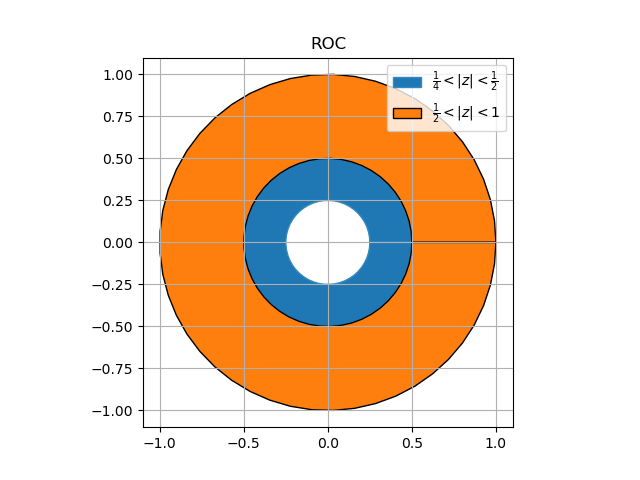
\includegraphics[width=\columnwidth]{Graphs/ROC.png}
 \caption{ROC}
 \end{figure}
 
 \begin{figure}[!ht]
\centering
 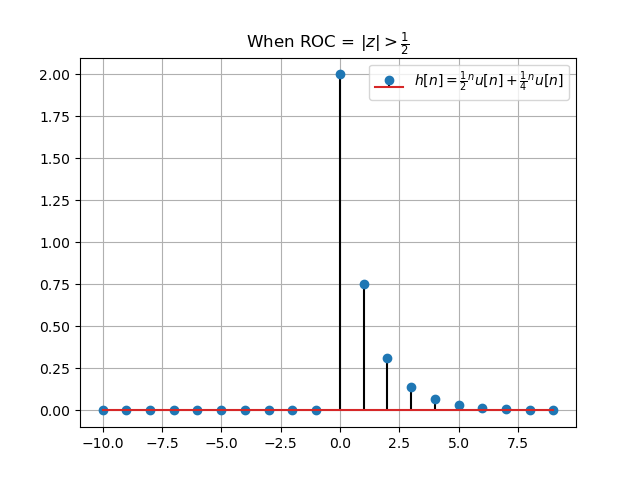
\includegraphics[width=\columnwidth]{Graphs/S1.png}
 \caption{$h[n]$ when $\abs{z} > \frac{1}{2}$}
 \end{figure}
  \begin{figure}[!ht]
\centering
 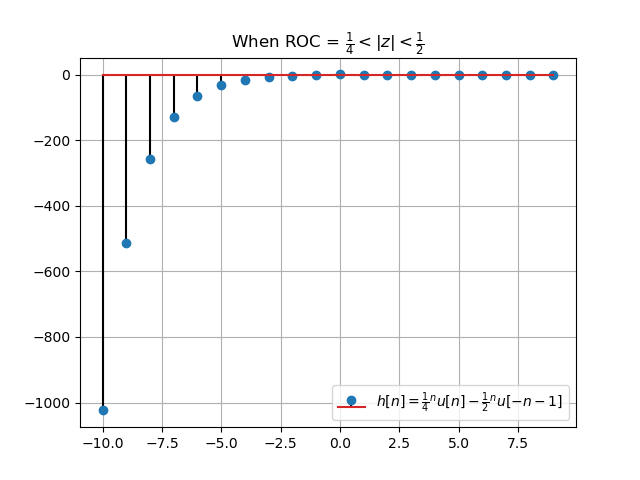
\includegraphics[width=\columnwidth]{Graphs/S3.png}
 \caption{$h[n]$ when $\frac{1}{4}<\abs{z} < \frac{1}{2}$}
 \end{figure}
  \begin{figure}[!ht]
\centering
 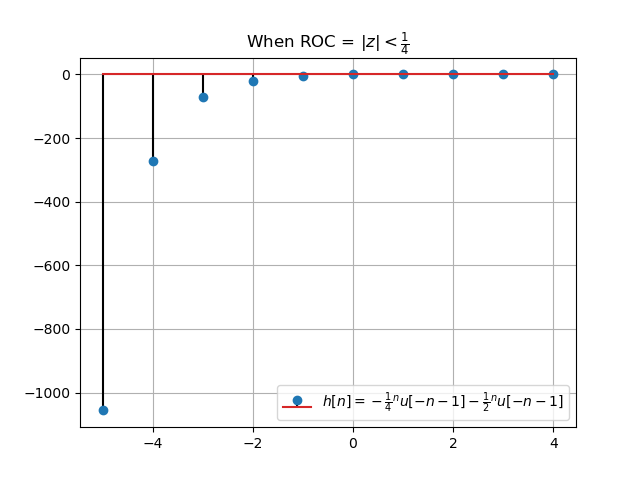
\includegraphics[width=\columnwidth]{Graphs/S2.png}
 \caption{$h[n]$ when $\abs{z} < \frac{1}{4}$}
 \end{figure}
 
 \end{document}